% !TEX root = /media/ueslei/Ueslei/INPE/PCI/Guia_COAWST/main.tex
\chapterimage{ocean2.jpg}
\chapter{Características do COAWST}

\noindent Até aqui aprendemos como utilizar o cluster Kerana e, de maneira tangencial, como compilar e rodar um simples caso teste do COAWST. A partir de agora entraremos nas especificidades dos modelos, como por exemplo, alterar o número de processadores utilizados e a taxa de troca de informações entre eles.
\bigskip

\section{Os arquivos estruturais dos modelos}
\bigskip

\noindent Como você pode ter notado ao simular o caso Sandy, os modelos possuem arquivos gerenciais que auxiliam o usuário na definição do projeto:
\bigskip

\noindent O ROMS utiliza o arquivo \textit{sandy.h} como arquivo que contém as opções de pré-processamento de C que definem o projeto. Acesse o site \textcolor{bleu_cite}{\textit{https://www.myroms.org/wiki/cppdefs.h}} para conhecer as definições disponíveis para o arquivo. O ROMS também utiliza o \textit{ocean\_sandy.in} como entrada padrão para executar o modelo. Este arquivo define as dimensões espaciais do projeto e parâmetros que não são informados durante a compilação, como por exemplo o passo de tempo, coeficientes e constantes físicas, configuração de coordenadas verticais, sinalizadores para controlar a frequência de saída, entre outros fatores. É possível aprender mais sobre este arquivo acessando o site \textcolor{bleu_cite}{\textit{https://www.myroms.org/wiki/ocean.in}}.
\bigskip

\noindent O WRF utiliza o arquivo \textit{namelist.input} como arquivo para gerenciar as informações sobre o projeto, bem como os esquemas de parametrizações serão utilizados. Para aprender sobre a descrição do arquivo, visite \textcolor{bleu_cite}{\textit{https://esrl.noaa.gov/gsd/wrfportal/namelist\_input\_options.html}}. Para aprender sobre as opções físicas do modelo e as referências de cada um deles, acesse  \textcolor{bleu_cite}{\textit{http://www2.mmm.ucar.edu/wrf/users/phys\_references.html}}.
\bigskip

\noindent O SWAN utiliza o arquivo \textit{swan\_sandy.in} como gerenciador. Nele estão descritos diversos parâmetros, como a descrição do projeto, os dados de entrada, de grade e de condições de fronteira e iniciais, as parametrizações físicas de ondas, entre outros. Para saber mais sobre como configurar o arquivo, visite a guia \textit{User Manual} no site \textcolor{bleu_cite}{\textit{http://swanmodel.sourceforge.net/}} e procure pela seção \textit{Description of commands}.
\bigskip

\section{Modificando o número de processadores}
\bigskip

\subsection{Modificando os processadores no ROMS}
\bigskip

\noindent No ROMS, os processadores estão localizados no arquivo \textit{ocean.in}, que fica dentro da pasta \textit{Projects}, e se chamam \textit{NtileI} e \textit{NtileJ}. Um exemplo está na Figura \textcolor{bleu_cite}{\ref{romsproc}}. Neste caso o ROMS reservará 160 processadores para ser executado, pois 16 x 10 = 160.
\bigskip

\begin{figure}[H]
    \centering
    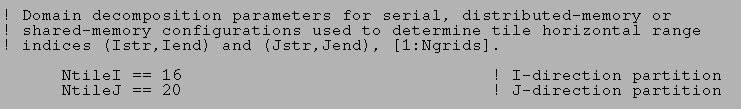
\includegraphics[width=0.80\textwidth]{roms_proc.png}
    \caption{Representação do número de processadores usados no ROMS.}
    \label{romsproc}
\end{figure}
\bigskip

\subsection{Modificando os processadores no WRF}
\bigskip

\noindent Para alterar o número de processadores do WRF é necessário modificar o arquivo \textit{namelist.input}. Nele existem as variáveis \textit{nproc\_x} e \textit{nproc\_y}, como na Figura \textcolor{bleu_cite}{\ref{procswrf}}. Neste caso serão reservados 320 processadores para o modelo atmosférico.
\bigskip

\begin{figure}[H]
    \centering
    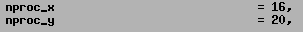
\includegraphics[width=0.50\textwidth]{wrf_proc.png}
    \caption{Representação do número de processadores para o WRF.}
    \label{procswrf}
\end{figure}
\bigskip

\subsection{Modificando os processadores no SWAN}

\bigskip O arquivo \textit{.in} do SWAN não discrimina os números de processadores usados, portanto basta alterar o número de processadores dele no \textit{coupling.in}, como será mostrado na subseção a seguir.
\bigskip

\subsection{Modificando os processadores no COAWST}
\bigskip

\noindent Agora que foram modificados, individualmente, o número de processadores que serão utilisados pelos modelos, o acoplador precisa ser informado sobre esta quantidade de processadores. Essa informação é passeda no arquivo \textit{coupling.in}. Dentro dele deverão constar o número total de processadores a serem utilizados pelos modelos ROMS, WRF e SWAN, como na Figura \textcolor{bleu_cite}{\ref{procscoa}}:
\bigskip

\begin{figure}[H]
    \centering
    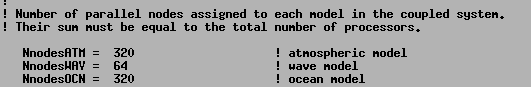
\includegraphics[width=0.80\textwidth]{taxa_acopl.png}
    \caption{Representação do número de processadores para cada módulo do COAWST.}
    \label{procscoa}
\end{figure}
\bigskip

\noindent O \textit{NnodesATM} é referente ao total de processadores utilizados pelo WRF, o \textit{NnodesWAV} é o total do SWAN e o \textit{NnodesOCN} o do ROMS. Basta mudar de acordo com o total de processadores utilizados nos passos anteriores.
\bigskip

\noindent Por fim, é preciso modificar o total de processadores no \textit{run.sh}, usado para submeter o experimento. Some o total de processadores usados pelos três modelos, seguindo a Equação \textcolor{bleu_cite}{\ref{equacao2}}:
\bigskip

\begin{equation}
TotalProc = NnodesATM + NnodesWAV + NnodesOCN
\label{equacao2}
\end{equation}
\bigskip

\noindent Onde  \textit{NnodesATM} é o número de processadores utilizados no WRF, \textit{NnodesWAV} o número de processadores no SWAN, \textit{NnodesOCN} o total de processadores no ROMS e \textit{TotalProc} a soma de todos os processadores usados nos modelos.
\bigskip

\noindent Agora abra o arquivo \textit{run.sh}, localizado dentro da pasta \textit{Work}, e procure pelas linhas a seguir:
\bigskip

\begin{bashcode}
\# PBS -l mppwidth=3
aprun -n 3 coawstM ./coupling.in 1> log.out 2> log.err
\end{bashcode}
\bigskip

\noindent Modifique o número \textit{3} pelo número total de processadores utilizados.
\bigskip

\section{Modificando o intervalo de tempo do acoplamento entre os modelos}
\bigskip

\noindent Para modificar o intervalo de troca de informações entre os modelos, abra o arquivo \textit{coupling.in} e modifique as variáveis \textit{TI\_ATM2WAV}, \textit{TI\_ATM2OCN}, \textit{TI\_WAV2ATM}, \textit{TI\_WAV2OCN}, \textit{TI\_OCN2WAV}, \textit{TI\_OCN2ATM}, como na Figura \textcolor{bleu_cite}{\ref{taxaacopla}}.
\bigskip

\begin{tcolorbox}[enhanced,
  grow to left by=0cm,%   equivalent to negative mdframed 'leftmargin'
  grow to right by=0cm,%  equivalent to negative mdframed 'rightmargin'
  enlarge top by=0cm,%     equivalent to mdframed 'skipabove'
  enlarge bottom by=0cm,%  equivalent to mdframed 'skipbelow'
  tcbox raise base,
  boxrule=1.0pt,
  left=18mm,
  colframe=red!50!black,coltext=red!25!black,colback=red!10!white,
  overlay={\begin{tcbclipinterior}\fill[red!75!blue!50!white] (frame.south west)
    rectangle node[text=white,font=\sffamily\bfseries\footnotesize,rotate=0] {ATENÇÃO} ([xshift=18mm]frame.north west);\end{tcbclipinterior}}]
A taxa de troca de informações deverá ser escolhida em segundos.
\end{tcolorbox}
\bigskip

\begin{figure}[H]
    \centering
    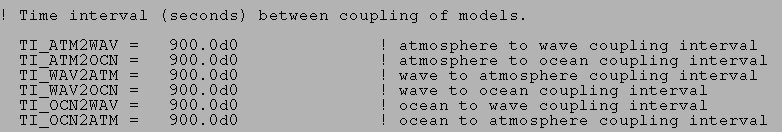
\includegraphics[width=0.95\textwidth]{coupltime.png}
    \caption{Intervalo de troca de informações entre os modelos utilizados no COAWST. Neste exemplo, a troca ocorrerá a cada 900 segundos.}
    \label{taxaacopla}
\end{figure}
\bigskip
